\documentclass[12pt]{article} \setlength{\oddsidemargin}{0in}
\setlength{\evensidemargin}{0in} \setlength{\textwidth}{6.5in}
\setlength{\parindent}{0in} \setlength{\textwidth}{16cm}
\setlength{\topmargin}{1in} \addtolength{\topmargin}{-1.5in}
\setlength{\textheight}{23cm} \setlength{\parskip}{0.75cm}

% Brackets
\usepackage{mathtools} \DeclarePairedDelimiter\ceil{\lceil}{\rceil}
\DeclarePairedDelimiter\floor{\lfloor}{\rfloor}

% Tikz settings
\usepackage{tikz} \usetikzlibrary{trees} \usetikzlibrary {positioning}
\definecolor {mypurple}{cmyk}{0.6,0.4,0.1,0} \definecolor
{myred}{cmyk}{0,0.3,0.3,0} \usetikzlibrary{fit,shapes.misc}

% Typesetting options
\usepackage{fancyvrb} \usepackage{amsmath,amsfonts,amssymb}
\usepackage [english]{babel} \usepackage [autostyle, english =
american]{csquotes} \usepackage[none]{hyphenat} \usepackage{url}

\usepackage{listings}
\usepackage{float}

\begin{document}

\noindent CSCI 3104 Spring 2018 \hfill Problem Set 9\\
Cole Schlisner (04/12)

% Image
\graphicspath{ {images/} }

\hrulefill

{\fontfamily{cmr}\selectfont}

% ******************* PROBLEM 1 *********************
\section*{Problem 1}

\textit{(10 pts) Let $G = (V, E)$ be a graph with an edge-weight function $w$, and let the tree
$T \subseteq E$ be a minimum spanning tree on $G$. Now, suppose that we modify $G$ slightly by
decreasing the weight of exactly one of the edges in $(x, y) \in T$ in order to produce a
new graph $G'$. Here, you will prove that the original tree $T$ is still a minimum spanning
tree for the modified graph $G'$.}

\textit{To get started, let $k$ be a positive number and define the weight function $w'$ as}

$$
w'(u,v) =
  \begin{cases}
    w(u,v) & \text{if $(u,v) \ne (x,y)$} \\
    w(u,v)-k & \text{if $(u,v) = (x,y)$}
  \end{cases}
  $$

\textit{Now, prove that the tree $T$ is a minimum spanning tree for $G'$, whose edge weights are
given by $w'$.}

Because $(x,y) \in T$, decreasing the weight of the edge $(x,y)$ only reaffirms the solution T. In other words, because the minimum path from vertex x to vertex y in G was the edge (x,y), decreasing the weight of that edge cannot make it cost more than another path (and thus change the solution). What this could do is decrease the \textit{amount} of MSTs for G` -- for example if T was one of two equivalent MSTs for G, then decreasing the weight of one of the edges in T makes it a unique solution as it now has a lower cost than the other spanning tree. 

\newpage

% ******************* PROBLEM 2 *********************
\section*{Problem 2}

\textit{(20 pts) Professor Snape gives you the following unweighted graph and asks you to
construct a weight function $w$ on the edges, using positive integer weights only, such
that the following conditions are true regarding minimum spanning trees and single-source shortest path trees:}
\begin{itemize}
\item The MST is distinct from any of the seven SSSP trees.
\item The order in which Jarnı́k/Prim’s algorithm adds the safe edges is different from the order in which Kruskal’s algorithm adds them.
\item Boru̇vka’s algorithm takes at least two rounds to construct the MST.
\end{itemize}

\textit{Justify your solution by (i) giving the edges weights, (ii) showing the corresponding
MST and all the SSSP trees, and (iii) giving the order in which edges are added by
each of the three algorithms. (For Boru̇vka’s algorithm, be sure to denote which edges
are added simultaneously in a single round.)}

\begin{figure}[h]
  \centering 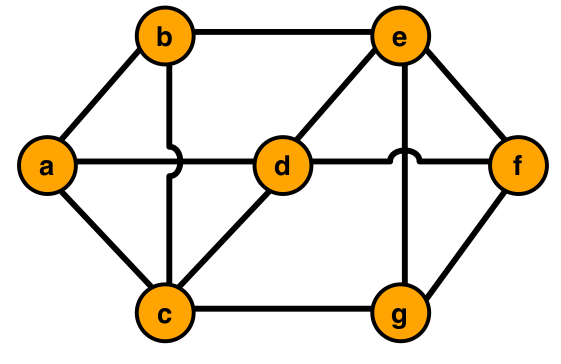
\includegraphics[width=0.5\textwidth]{P2}
\end{figure}

\newpage

\begin{enumerate}
  \item[\textbf{i.}]
    \textbf{Weights:}\\
    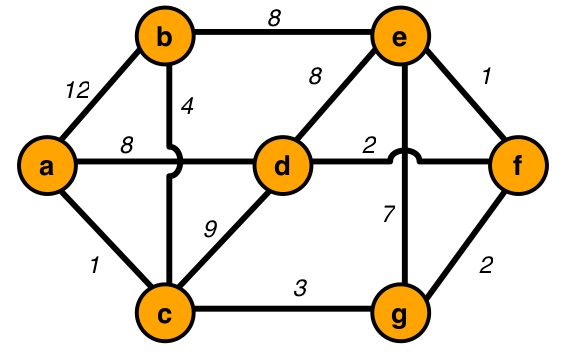
\includegraphics[width=0.4\textwidth]{P2-weights} \\
  \item[\textbf{ii.}]
    \textbf{MST:} \\
    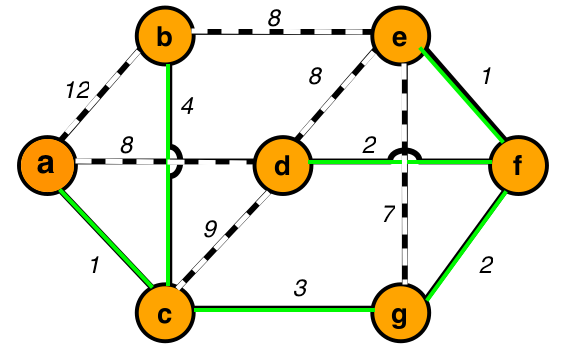
\includegraphics[width=0.4\textwidth]{P2-mst} \\
    \textbf{SSSPs 1-7:} \\
    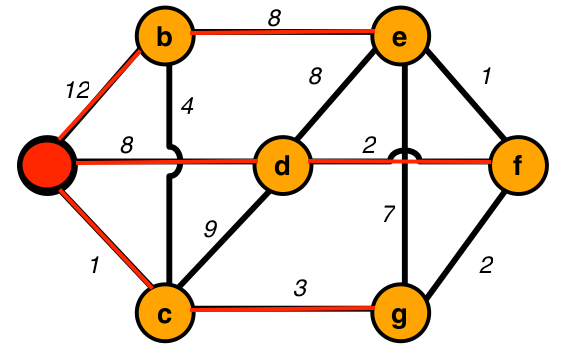
\includegraphics[width=0.4\textwidth]{P2-sssp1}
    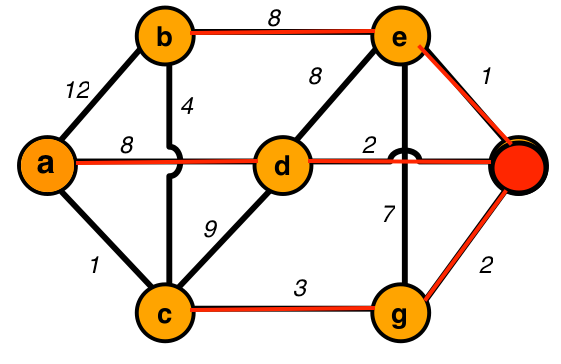
\includegraphics[width=0.4\textwidth]{P2-sssp2}\\
    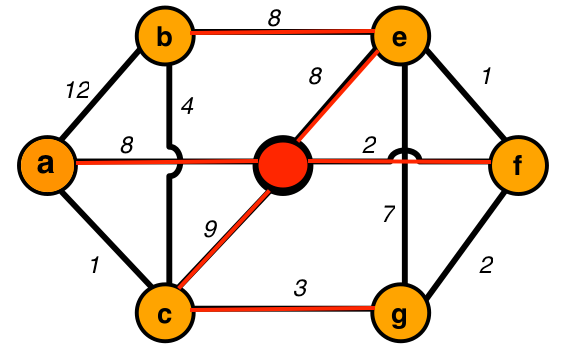
\includegraphics[width=0.4\textwidth]{P2-sssp3}
    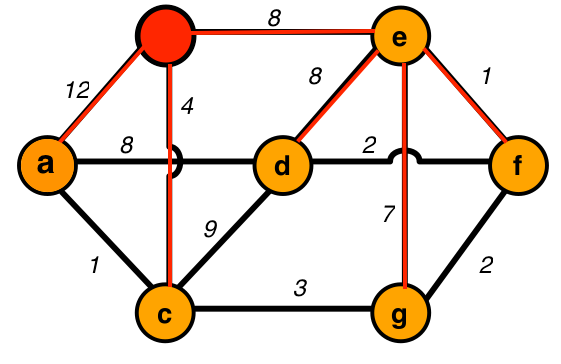
\includegraphics[width=0.4\textwidth]{P2-sssp4}\\
    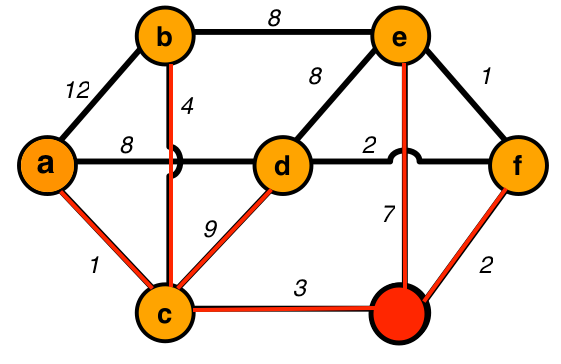
\includegraphics[width=0.4\textwidth]{P2-sssp5}
    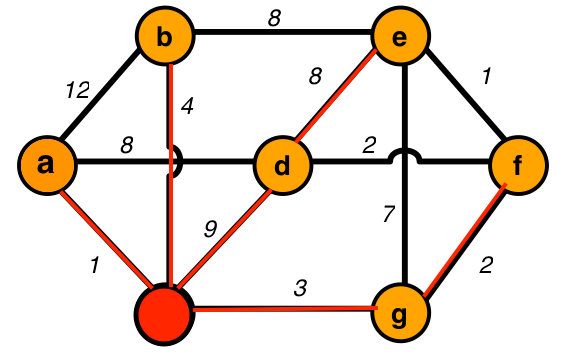
\includegraphics[width=0.4\textwidth]{P2-sssp6}\\
    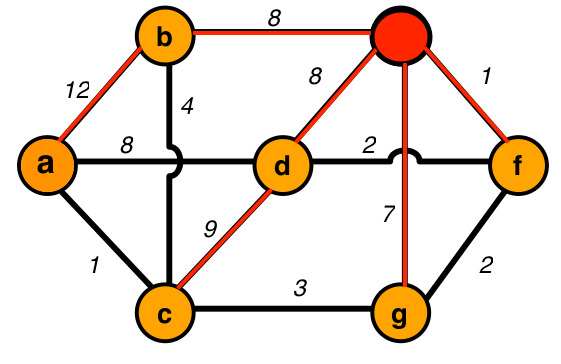
\includegraphics[width=0.4\textwidth]{P2-sssp7}
  \item[\textbf{iii.}]
    \textbf{Prim:} \\
    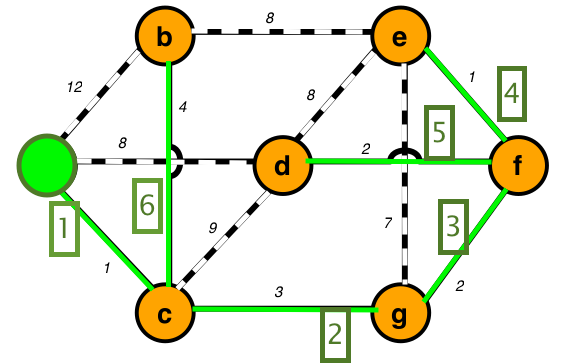
\includegraphics[width=0.4\textwidth]{P2-prim}\\
    \textbf{Kruskal:}\\
    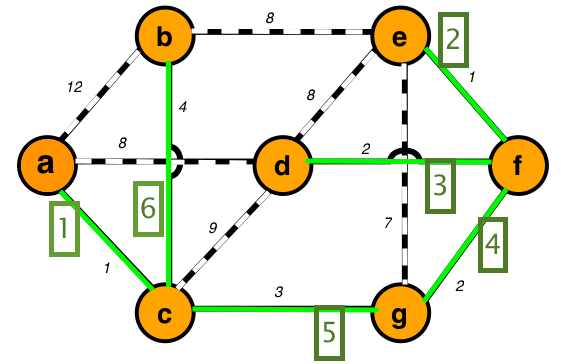
\includegraphics[width=0.4\textwidth]{P2-kruskal}\\
    \newpage
    \textbf{Boruvka:}\\
    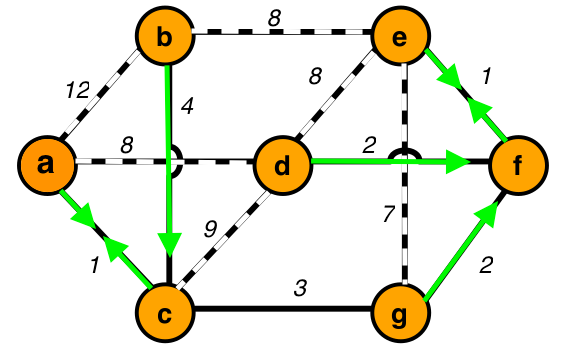
\includegraphics[width=0.4\textwidth]{P2-boruvka1}\\
    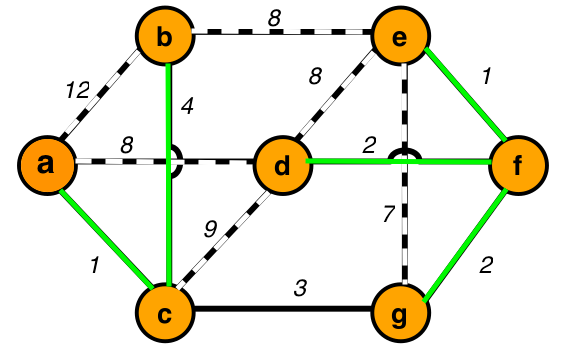
\includegraphics[width=0.4\textwidth]{P2-boruvka2}\\
    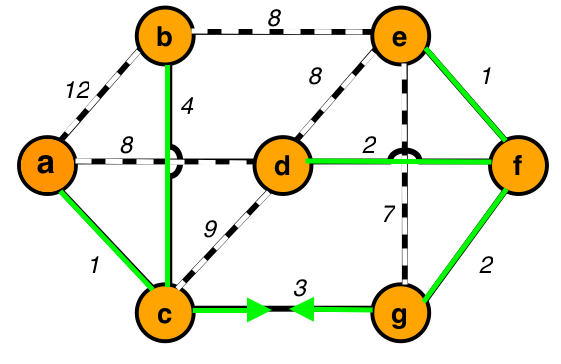
\includegraphics[width=0.4\textwidth]{P2-boruvka3}\\
    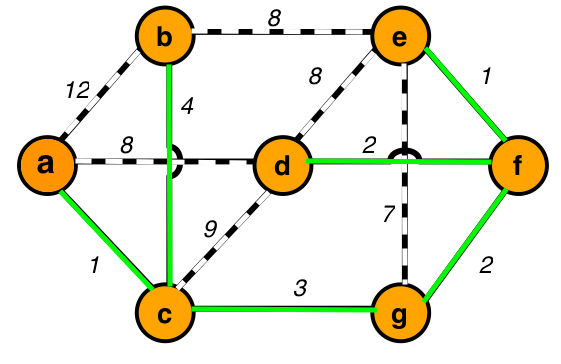
\includegraphics[width=0.4\textwidth]{P2-boruvka4}
\end{enumerate}
\newpage

% ******************* PROBLEM 3 *********************
\section*{Problem 3}

\textit{(10 pts extra credit) Crabbe and Goyle think they have come up with a way to get
rich by playing the foreign exchange markets in the wizarding world. Their idea is
to exploit these exchange rates in order to transform one unit of British wizarding
money into more than one unit of British wizarding money. For instance, suppose
1 wizarding penny bought 0.82 French wizarding pennies, 1 French wizarding penny
bought 129.7 Russian wizarding pennies, 1 Russian wizarding penny, and one Russian
wizarding penny bought 0.0008 British wizarding pennies. By converting these coins,
Crabbe and Goyle think they could start with 1 British wizarding penny and buy
$0.82 \times 129.7 \times 12 \times 0.0008 \approx 1.02$ British wizarding pennies, thereby making a $2\%$
profit! The problem is that those gnomes at Gringots charge a transaction cost for
each exchange...}

\textit{Suppose that Crabbe and Goyle start with knowledge of $n$ wizard monies $c_1, c_2, \cdots, c_n$
and an $n \times n$ table $R$ of exchange rates, such that one unit of wizard money $c_i$ buys
$R[i, j]$ units of wizard money $c_j$. A traditional \textbf{arbitrage opportunity} is thus a cycle
in the induced graph such that the product of the edge weights is greater than unity.
That is, a sequence of currencies $\langle c_{i_{1}}, c_{i_{2}} , \cdots , c_{i_{k}} \rangle$ such that $R[i_1, i_2] \times R[i_2, i_3] \times \cdots \times R[i_{k−1}, i_k] \times R[i_k, i_i] > 1$. Each transaction, however, must pay Gringots a fraction $\alpha$ of the total transaction value, e.g., $\alpha = 0.01$ for a $1\%$ rate.}

\begin{enumerate}
\item[(a)]{\textit{When given $R$ and $\alpha$, give an efficient algorithm that can determine if an arbitrage opportunity exists. Analyze the running time of your algorithm.}

    \textit{Hermione’s hint: It is possible to solve this problem in O(n 3 ). Recall that Bellman-Ford can be used to detect negative-weight cycles in a graph.}
  }
  \\\\
  TODO
  \\
\item[(b)]{\textit{For an arbitrary $R$, explain how varying $\alpha$ changes the set of arbitrage opportunities that exist and that your algorithm might identify.}}
  \\\\
  TODO

\end{enumerate}

\newpage
% ******************* PROBLEM 4 *********************
\section*{Problem 4}

\textit{(40 pts) Bidirectional breadth-first search is a variant of standard BFS for finding a
shortest path between two vertices $s, t \in V(G)$. The idea is to run two breadth-first
searches simultanesouly, one starting from $s$ and one starting from $t$, and stop when
they “meet in the middle” (that is, whenever a vertex is encountered by both searches).
``Simultaneously'' here doesn’t assume you have multiple processors at your disposal;
it’s enough to alternate iterations of the searches: one iteration of the loop for the BFS
that started at $s$ and one iteration of the loop for the BFS that started at $t$.}

\textit{As we’ll see, although the worst-case running time of BFS and Bidirectional BFS are
asymptotically the same, in practice Bidirectional BFS often performs significantly
better.}

\textit{Throughout this problem, all graphs are unweighted, undirected, simple graphs.}
\\\\

\begin{enumerate}
\item[(a)]{\textit{Give examples to show that, in the worst case, the asymptotic running time of
bidirectional BFS is the same as that of ordinary BFS. Note that because we are
asking for asymptotic running time, you actually need to provide an infinite family
of examples $(G_n , s_n , t_n )$ such that $s_n, t_n \in V(G_n)$, the asymptotic running time of
BFS and bidirectional BFS are the same on inputs $(G_n, s_n, t_n)$, and $|V(G_n)| \rightarrow \infty$ as $n \rightarrow \infty$}}
  \\\\
  I don't know how to answer this.
  \\
  \pagebreak
\item[(b)]{\textit{Recall that in ordinary BFS we used a \texttt{state} array (see Lecture Notes 8) to keep track of which nodes had been visited before. In bidirectional BFS we will need two
\texttt{state} arrays, one for the BFS from $s$ and one for the BFS from $t$. Why? Give an
example to show what can go wrong if there’s only one state array. In particular,
give a graph $G$ and two vertices $s, t$ such that some run of a bidirectional BFS
says there is no path from $s$ to $t$ when in fact there is one.}}
  \\\\
  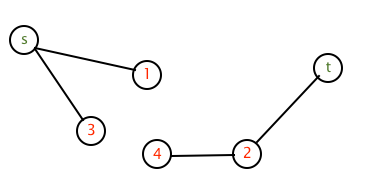
\includegraphics[width=0.4\textwidth]{P4-b} \\
  In this diagram, each red number indicates the order in which a given node was marked as "old" by either the BFS tree growing from vertex s or the BFS tree growing from t. The tree growing from s would next attempt to explore the vertex marked "4", but it can't because it was marked as "old" by the BFS tree from t. Thus, the algorithm with one state array would not find a path between s and t. 
  \newpage
  \item[(c)]{\textit{Implement from scratch a function \texttt{BFS(G,s,t)} that performs an ordinary BFS in the (unweighted, directed) graph G to find a shortest path from s to t. Assume
the graph is given as an adjacency list; for the list of neighbors of each vertex,
you may use any data structure you like (including those provided in standard
language libraries). Have your function return a pair $(d, k)$, where $d$ is the distance
from $s$ to $t$ ($-1$ if there is no $s$ to $t$ path), and $k$ is the number of nodes popped
off the queue during the entire run of the algorithm.}}
  \\\\
  \begin{verbatim}
  def BFS(g, s, t):
    # distance can't be more than 2|V|
    dist = [len(g)*2 for i in range(len(g))]
    # False = NEW, True = OLD
    old = [False for i in range(len(g))]

    dist[s] = 0

    Q = [(None, s)]

    d = 0
    
    while (len(Q) > 0):
      # dequeue u,v   
      (u,v) = Q.pop(0)
      d += 1

      if not old[v]:
        old[v] = True
      
        if u is not None:
          dist[v] = dist[u] + 1
      
        # add all neighbors of v
        for i in range(len(g)):
          if g[v][i]:
            if i == t:
              return (dist[v]+1, d)
            Q.append((v, i))
    return (-1, d)
  \end{verbatim}
  \newpage
\item[(d)]{\textit{Implement from scratch a function \texttt{BidirectionalBFS(G,s,t)} that takes in an (unweighted, directed) graph $G$, and two of its vertices $s,t$, and performs a bidirectional BFS. As with the previous function, this function should return a pair
$(d, k)$ where $d$ is the distance from $s$ to $t$ ($-1$ if there is no path from $s$ to $t$) and $k$ is the number of vertices popped off of both queues during the entire run of the
algorithm.}}
  \\\\
  The next two pages contain a complete Python (3.5) program containing the function, as well as a function to generate an arbitrary sized directed graph for testing. (Assume page break preserves indentation) \pagebreak
  \begin{verbatim}
  import random as r
  import numpy as np

  def bidirectionalBFS(g, s, t):
    # distance can't be more than 2|V|
    Sdist = [len(g)*2 for i in range(len(g))]
    Tdist = [len(g)*2 for i in range(len(g))]
    # False = NEW, True = OLD
    Sstate = [False for i in range(len(g))]
    Tstate = [False for i in range(len(g))]

    Sdist[s] = 0
    Tdist[t] = 0

    SQ = [(None, s)]
    TQ = [(None,t)]

    d = 0
    
    # keep track of which tree we are growing
    S_BFS = True
    while (len(SQ) > 0 and len(TQ) > 0):
      # choose which state/dist/queue to use
      old = Sstate if S_BFS else Tstate
      dist = Sdist if S_BFS else Tdist
      Q = SQ if S_BFS else TQ

      # dequeue u,v   
      (u,v) = Q.pop(0)
      d += 1

      if not old[v]:
        old[v] = True
      
        if u is not None:
          dist[v] = dist[u] + 1
      
        # if v was marked as old by other tree, there is a path
        if (S_BFS and Tstate[v]) or (not S_BFS and Sstate[v]):
          return (Tdist[v]+Sdist[v], d)
        
        # add all neighbors of v
        for i in range(len(g)):
          if g[v][i]:
            # if the node we are looking for is a neighbor, there is a path
            if i == (t if S_BFS else s):
              return (dist[v]+1, d)
            Q.append((v, i))
        
        S_BFS = not S_BFS
    
    return (-1, d)

  """
    Generates (n * n) boolean matrix where:
      (g[1][2] == True) => there is a directed edge from vertex 1 to vertex 2
  """
  def generate_directed_graph(n):
    g = [[r.choice([True,False]) for i in range(n)] for j in range(n)]
    # remove all self loops
    for i in range(n):
      g[i][i] = False

    return g

  G = generate_directed_graph(7)
  print(np.array(G))
  print(bidirectionalBFS(G,0,6))
  \end{verbatim}
  \newpage
\item[(e)]{\textit{For each of the following families of graphs $G_n$ , write code to execute BFS and BidirectionalBFS on these graphs, and produce the following output:}
    \begin{itemize}
    \item \textit{In text, the tuples $(n, d_1, k_1, d_2, k_2)$ where $n$ is the index of the graph, $(d_1, k_1)$ is the output of \texttt{BFS} and $(d_2, k_2)$ is the output of \texttt{BidirectionalBFS}.}
    \item \textit{a plot with $n$ on the x-axis, $k$ on the y-axis, and with two line charts, one for the values of $k_1$ and one for the values of $k_2$:}
    \end{itemize}
    \begin{enumerate}
    \item[i.] \textit{Grids. $G_n$ is an $n \times n$ grid, where each vertex is connected to its neighbors in the four cardinal directions $(N,S,E,W)$. Vertices on the boundary of the grid
will only have 3 neighbors, and corners will only have 2 neighbors. Let $s_n$
be the midpoint of one edge of the grid, and $t_n$ the midpoint of the opposite
edge. For example, for $n = 3$ we have:}

\begin{figure}[h]
  \centering 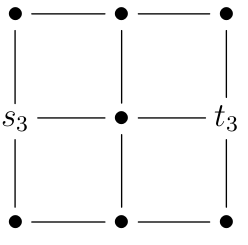
\includegraphics[width=0.3\textwidth]{P41}
\end{figure}

\textit{Produce output for $n = 3, 4, 5, \cdots, 20$.}

\item[ii.] \textit{Trees. $G_n$ is a complete binary tree of depth $n$. $s_n$ is the root and $t_n$ is any leaf. Produce output for $n = 3, 4, 5, \cdots, 15$. For example, for $n = 3$ we have:}

  \begin{figure}[H]
  \centering 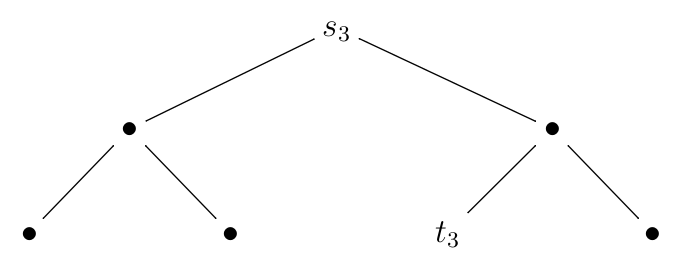
\includegraphics[width=1\textwidth]{P42}
  \end{figure}

\item[iii.] \textit{Random graphs. $G_n$ is a graph on $n$ vertices constructed as follows. For each
pair of of vertices $(i, j)$, get a random boolean value; if it is true, include
the edge $(i, j)$, otherwise do not. Let $s_n$ be vertex 1 and $t_n$ be vertex 2 (food
for thought: why does it not matter, on average, which vertices we take $s, t$
to be?) For each $n$, produce 50 such random graphs and report just the
average values of $(d_1, k_ 1, d_2, k_2 )$ over those 50 trials. Produce this output for $n = 3, 4, 5, \cdots, 20$.}
    \end{enumerate}
  }

  I don't know

\end{enumerate}



% ---------------------------------------------------
\end{document}
